\documentclass[tikz]{standalone}
%\usepackage{fontawesome}

% \newfontfamily{\FA}{Font Awesome 5 Free} % some glyphs missing
\expandafter\def\csname faicon@facebook\endcsname{{\FA\symbol{"F09A}}}
\def\faQuestionSign{{\FA\symbol{"F059}}}
\def\faQuestion{{\FA\symbol{"F128}}}
\def\faExclamation{{\FA\symbol{"F12A}}}
\def\faUploadAlt{{\FA\symbol{"F093}}}
\def\faLemon{{\FA\symbol{"F094}}}
\def\faPhone{{\FA\symbol{"F095}}}
\def\faCheckEmpty{{\FA\symbol{"F096}}}
\def\faBookmarkEmpty{{\FA\symbol{"F097}}}

%\def\faCatt{{\FA\symbol{"F6BE}}}
%\def\faCat{\faicon{cat}}
%\def\faCat{\faicon{yoast}}
\expandafter\def\csname faicon@dog\endcsname{{\FA\symbol{"F4DA}}}
%\def\faDog{\faicon{dog}}
%\def\faDog{{\FA\symbol{"F4DA}}}
%\def\faDogg{{\FA\symbol{"F6D3}}}
%\def\faDogg{{\FA\symbol{"F596}}}

% /usr/share/texlive/texmf-dist/fonts/opentype/public/fontawesome5/FontAwesome5Free-Solid-900.otf
\newfontfamily{\FAS}{FontAwesome5Free-Solid-900.otf}
%\expandafter\def\csname faicon@download\endcsname{{\FAS\symbol{"F6D3}}}
\expandafter\def\csname faicon@cat\endcsname{{\FAS\symbol{"F6BE}}}
\def\faCat{\faicon{cat}}
\expandafter\def\csname faicon@dog\endcsname{{\FAS\symbol{"F6D3}}}
\def\faDog{\faicon{dog}}
\expandafter\def\csname faicon@dragon\endcsname{{\FAS\symbol{"F6D5}}}
\def\faDragon{\faicon{dragon}}
\expandafter\def\csname faicon@fish\endcsname{{\FAS\symbol{"F578}}}
\def\faFish{\faicon{fish}}
\expandafter\def\csname faicon@horse\endcsname{{\FAS\symbol{"F6F0}}}
\def\faHorse{\faicon{horse}}
\expandafter\def\csname faicon@spider\endcsname{{\FAS\symbol{"F717}}}
\def\faSpider{\faicon{spider}}

\expandafter\def\csname faicon@chessking\endcsname{{\FAS\symbol{"F43F}}}
\def\faChessKing{\faicon{chessking}}
\expandafter\def\csname faicon@chessqueen\endcsname{{\FAS\symbol{"F445}}}
\def\faChessQueen{\faicon{chessqueen}}
\expandafter\def\csname faicon@chessrook\endcsname{{\FAS\symbol{"F447}}}
\def\faChessRook{\faicon{chessrook}}
\expandafter\def\csname faicon@chesspawn\endcsname{{\FAS\symbol{"F443}}}
\def\faChessPawn{\faicon{chesspawn}}
\expandafter\def\csname faicon@chessknight\endcsname{{\FAS\symbol{"F441}}}
\def\faChessKnight{\faicon{chessknight}}
\expandafter\def\csname faicon@chessbishop\endcsname{{\FAS\symbol{"F43A}}}
\def\faChessBishop{\faicon{chessbishop}}
\expandafter\def\csname faicon@chess\endcsname{{\FAS\symbol{"F439}}}
\def\faChess{\faicon{chess}}







\usepackage{tikz}
\usetikzlibrary{positioning,trees,decorations.pathreplacing}

\begin{document}
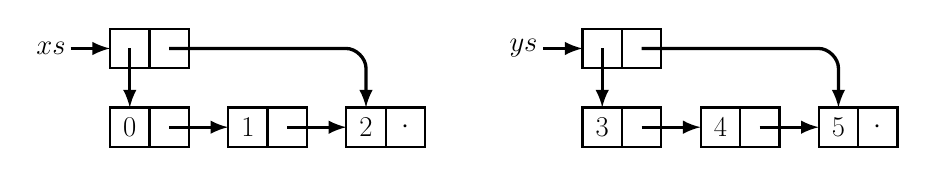
\begin{tikzpicture}[thick,scale=0.5, every node/.style={scale=0.5}]
    \tikzstyle{marrs}=[very thick,-latex]

    \begin{scope}
    
        \foreach \x/\y in {0/0, 0/-2, 3/-2, 6/-2} {
            \draw (\x - 0.5, \y - 0.5) rectangle +(1, 1); \draw (\x + 1 - 0.5, \y - 0.5) rectangle +(1, 1);
        }
        \draw[marrs] (-1.5, 0) -> +(1, 0);
        \draw[marrs] (0, 0) -> +(0, -1.5);
        \draw[marrs] (1, -2) -> +(1.5, 0);
        \draw[marrs] (4, -2) -> +(1.5, 0);
        \draw[marrs] (1, 0) -- (5.5, 0) .. controls (5.75, 0) and (6, -0.25) .. (6, -0.5) -- (6, -1.5);
        
        { \huge
            \draw (-2, 0) node {$xs$};
            \draw (0, -2) node {$0$};
            \draw (3, -2) node {$1$};
            \draw (6, -2) node {$2$};
            \draw (7, -2) node {$\cdot$};
        }
    
    \end{scope}
    
    \begin{scope}[xshift=12cm]
    
        \foreach \x/\y in {0/0, 0/-2, 3/-2, 6/-2} {
            \draw (\x - 0.5, \y - 0.5) rectangle +(1, 1); \draw (\x + 1 - 0.5, \y - 0.5) rectangle +(1, 1);
        }
        \draw[marrs] (-1.5, 0) -> +(1, 0);
        \draw[marrs] (0, 0) -> +(0, -1.5);
        \draw[marrs] (1, -2) -> +(1.5, 0);
        \draw[marrs] (4, -2) -> +(1.5, 0);
        \draw[marrs] (1, 0) -- (5.5, 0) .. controls (5.75, 0) and (6, -0.25) .. (6, -0.5) -- (6, -1.5);
        
        { \huge
            \draw (-2, 0) node {$ys$};
            \draw (0, -2) node {$3$};
            \draw (3, -2) node {$4$};
            \draw (6, -2) node {$5$};
            \draw (7, -2) node {$\cdot$};
        }
    \end{scope}
\end{tikzpicture}
\end{document}